%!TEX root = ../dokumentation.tex
\chapter{Speech-To-Text-Konvertierung}


\section{Der Android Speech Recognition Client}
Der Android Speech Recognition Client verwendet die Androideigene Methode zur Spracherkennung.\\
Wird der Start Recording Button gedrückt, wird ein so genanntes SPEECH\_RECOGNITION\_INTENT gestartet, welches das Android Spracherkennungsprogramm mit der vom User gewählten Eingabesprache startet.
Die Android Spracherkennung arbeitet offline und asynchron. Zwar ist die offline Aktivität von vorteil, da der User keine aktive Datenverbindung benötigt, allerdings vermindert die asynchronität des Programms die Usability bei längeren Spracheingaben.\\
Hat der User die Spracheingabe beendet, wird die gesprochene Sprache in Text konvertiert und das Ergebnis als String an die Methode onReceiveResult() gesendet. Diese Methode überprüft, von welchem Intent das empfangene Ergebnis stammt und ist der Sender die Android Speech Recognition, so wird das Konvertierungsergebnis an die Methode receiveResult der MainActivity übergeben, welche die Darstellung auf dem verbundenem AR-Gerät verwaltet.\\
Wurde das Ergebnis übergeben, wird die stopRecording Funktionalität gestartet, welche die Applikation wieder in den Zustand vor einer Konvertierung versetzt.


\section{Speech-To-Text Konvertierung durch die Google Cloud API}
\paragraph{Aufbau des Moduls}
Die Klassen des Google Speech Recognition Moduls befinden sich im package de.dhbw.studienarbeit.hearItApp.recorder.googleSpeechRecognition. Zum aufzeichnen des Tons dient die Klasse VoiceRecorder welche das IRecorder Interface implementiert. Die Klasse VoiceRecorder wird der Klasse MainActivity als Recorder Instanz zugeordnet, wenn im User Interface die Google Speech Recognition als Option gewählt wurde. Sie implementiert die Interface Methoden startRecording(), stopRecording() und shutdown(). In ihrem Konstruktor wird die Klasse GoogleSpeechConverter instanziiert. Diese Klasse ist verantwortlich für die Konvertierung der vom VoiceRecorder aufgenommenen Audiodaten. Sie kommuniziert mit den Google Servern, sendet Audiodaten und empfängt das Konvertierungsergebnis.\\
Diese Komponenten werden im folgenden näher erläutert.
\\

\subsection{Der Voice Recorder}
Zur Aufnahme von Ton bietet Android zwei Optionen\cite{Recording Optionen}:
\begin{enumerate}
	\item Die Erste ist der Android Media Recorder. Dieser bietet ein einfaches Interface, um mit wenigen Code Zeilen eine Audio Aufnahme zu starten und die Audio Daten in eine Datei zu schreiben. Nach beendigung der Aufnahme kann die Datei abgespielt oder weiter verarbeitet werden.
	\item Die Zweite und für diesen Zweck passendere Methode ist die Audio Aufnahme durch ein Objekt der Klasse AudioRecord. Die Programmierung des AudioRecords findet eine Ebene tiefer statt, als die des MediaRecorders. Nachdem dem Objekt durch den Konstruktor die Aufnahmequelle, das Sampling, die Anzahl der Channels, das Encoding und die Buffergröße zugewiesen wurden, können nach dem Starten der Aufnahme in einer Schleife die aufgenommenen Audio Daten in Form von Byte oder Short Arrays ausgelesen werden.
\end{enumerate}
Ein Code-Beispiel zur Initialisierung und Aufnahme durch ein AudioRecord Objekt sieht so aus:
\begin{lstlisting}
AudioRecord androidRecord = new AudioRecord(MediaRecorder.AudioSource.MIC,
		VoiceRecorder.SAMPLING, VoiceRecorder.RECORDER_CHANNELS,
		VoiceRecorder.RECORDER_AUDIO_ENCODING, VoiceRecorder.BUFFER_SIZE);
		
androidRecord.startRecording();
boolean isRecording = true;

while (isRecording) {

	short[] shortBuffer = new short[VoiceRecorder.BUFFER_SIZE / 2];
	
	//read ist return code, shortBuffer der Buffer in den geschrieben wird
	int read = this.androidRecord.read(shortBuffer, 0, shortBuffer.length);
	
	//verarbeite auio daten in shortBuffer
	
}
\end{lstlisting}
\paragraph{Begrifflichkeiten}
Die im Konstruktor übergebenen Daten sind die Audioquelle, das Sampling, die Anzahl der Channels, das Encoding und die Buffergröße.\\
Die Audio Quelle ist das Gerät, von welchem Ton aufgezeichnet werden soll und die Anzahl der Channels gibt an, über wie viele Kanäle der Ton aufgenommen wird (Mono, Stereo, usw).\\
Unter dem Sampling versteht man die Anzahl der Werte die pro Sekunde aus dem Analogen Signal einer Audioquelle entommen werden sollen. Weil ein Analoges Signal eine Welle bestehend aus unendlich vielen Werten darstellt, muss das Signal zur digitalen Speicherung auf eine definierte Punktezahl reduziert werden. Diese Zahl nennt sich Sampling. Für dieses Projekt wurde ein 16 000 Sampling gewählt, da ein Kompromiss zwischen Übertragungszeit und Qualität gefunden werden musste. Je höher das Sampling, umso größer die Daten Menge, umso höher die Übertragungszeit.\\
Das Encoding gibt die Zahl der Bits an, die jeder gespeicherte Wert hat. Bei einem 16 Bit Encoding, hat jeder gespeicherte Wert eine größe von 2 Byte.\\
Die Buffergröße ist die Größe des Arrays, in welchen man die Daten später einliest. Die Buffergröße gibt an, wie viele Sekunden jeweils vom Mikrophon ausgelesen werden sollen.\\
Herleitung Buffer Größe:\\
Pro Schleifendurchlauf sollen 80 aufgezeichnete Millisekunden vom AudioRecord gelesen werden.\\
Ein Sampling von 16 000 mit Encoding 16 Bit, bedeutet, dass pro Sekunde 16 000 Werte a 16 Bit gespeichert werden, was 16 000 Werten von je 2 Byte also 32 000 Byte = 32 kByte enstspricht. Multipliziert man diesen Wert mit der gewünschten Aufnahme Zeit ergibt sich die Größe eines Buffers in Byte.\\
Die Speichergröße errechnet sich dann wie folgend:\\
\begin{equation}
Speichergröße = Sampling  * \frac{Encoding}{8} * Zeit \\
Speichergröße = 16 000 	  * \frac{16}{8} 	  * 0,8  = 25 600 Byte
\end{equation}
Nun kann also entweder ein Byte Array mit größe 25 600 an den AudioRecord übergeben werden, oder aber ein Short Array mit der halben größe, da  ein Short-Wert eine größe von 2 Byte hat.\\

\paragraph{Funktionaler Aufbau des Voice Recorders}
\begin{wrapfigure}{r}{0.4\linewidth}
	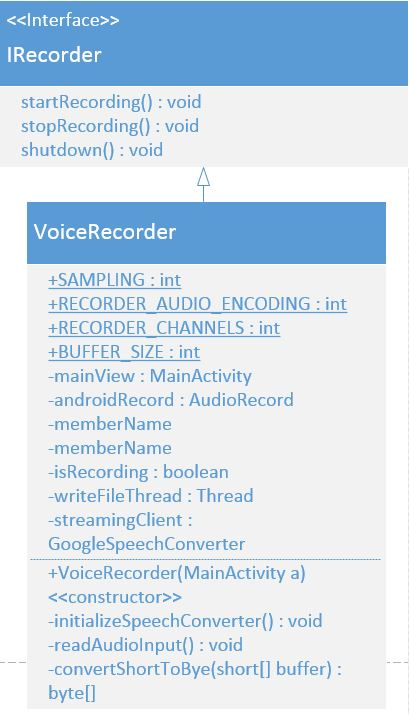
\includegraphics[width=\linewidth]{../images/VoiceRecorder.JPG}
	\caption{UML Klassendiagramm der Klasse VoiceRecorder}
	\label{fig:VoiceRecorder}
\end{wrapfigure}
Nachdem die Option Google Speech Conversion im User Interface gewählt wurde, wird durch die RecorderFactory Klasse eine Instanz des VoiceRecorders erzeugt. Im Konstruktor werden sowohl ein AudioRecord Objekt, als auch ein GoogleSpeechConverter Objekt, welches im Verlauf noch näher erläutert wird, inizialisiert. Danach steht der Recorder zur Verwendung bereit. \\
Wird im User Interface der Button zum starten der Konvertierung gedrückt, ruft die Klasse MainActivity die Methode startRecording() des Recorders auf. Innerhalb dieser Methode wird die Methode readAudioInput() der eigenen Klasse in einem eigenen Thread gestartet.\\
ReadAudioInput() setzt das Attribut isRecording auf true und beginnt eine while-Schleife, mit isRecording = false als Abbruchskriterium. Innerhalb der Schleife wird pro Durchlauf ein AudioBuffer mit Audio Daten gefüllt. Der Audio Buffer ist vom Typ short[]. Dieser Buffer wird der MainActivity-Methode showSoundAnimation übergeben, welche in Abhängigkeit der aus den Daten errechneten Lautstärke eine Animation erzeugt, um die laufende Aufnahme für den Benutzer zu visualisieren.\\
Danach wird  der short[]-Buffer durch die Methode convertShortToByte[] in einen byte[]-Buffer konvertiert und der Methode recognizeBytes der Klasse GoogleSpeechConverter übergeben, welche die Daten an Google sendet, um gesprochene Sprache zu erkennen und diese in Text zu konvertieren.\\
Die Konvertierung von short zu byte ist notwendig, da die Google Streaming Speech API lediglich byte[]-Buffer als Übergabewert akzeptiert. Die Methode showSoundAnimation verwertet allerdings short-Werte, da bei einem 16-Bit Encoding jeder einzelne Audiowert die länge von 2 byte, also einer short hat. Bei der Konvertierung wird jeder short-Wert im Buffer einmal mit 0x00FF maskiert  und das Ergebnis in einen byte-Array geschrieben. Die Maske 0x00FF setzt die oberen 8 Bit auf 0 und übernimmt die Werte der untern 8 Bit. Es bleibt eine 1 Byte große Zahl, welche den Wert der unteren Hälfte der short-Zahl hat. Danach wird die short-Zahl mit >> 8 um 8 Bit nach rechts geshiftet. Dies hat zur Folge, dass die untern 8 Bit verschwinden, während die oberen 8 Bit an die untere Stelle rücken. Die oberen 8 Bit werden mit nullen aufgefüllt. Wieder bleibt eine 8 Bit lange Zahl, welche die Werte der oberen Hälfte der short-Zahl enthält. Diese wird an die darauf folgende Stelle im byte-Buffer geschrieben.\\
Es entsteht ein Array der Form:
\begin{addmargin}[1cm]{0cm}
	buffer[0] = low Nibble Short[0]
	buffer[1] = high Nibble Short[0]
	buffer[2] = low Nibble Short[1]
	buffer[3] = high Nibble Short[1]
	...
\end{addmargin}
Quellcode der convertShortToByte-Methode:
\begin{lstlisting}
private byte[] convertShortToByte(short[] buffer) {

	byte[] byteBuffer = new byte[buffer.length * 2];

	for (int i = 0; i < buffer.length; i++) {
		//mask to set high 8 bit of short 0, let low 8 bit as is, add to array
		byteBuffer[i * 2] = (byte) (buffer[i] & 0x00FF);
		//shift right to get high 8 bit down, and add high bits to array
		byteBuffer[(i * 2) + 1] = (byte) (buffer[i] >> 8);
	}
return byteBuffer;

}
\end{lstlisting}
Wird der UI-Button zum Stoppen der Aufnahme gedrückt, oder passiert im Connector, GoogleSpeechConverter oder Recorder selbst ein schwerwiegende Fehler, wird die Recorder-Methode stopRecording() ausgeführt. Diese Methode Methode setzt das Attribut isRecording auf false, was zur Beendigung der Schleife führt. Auserdem wird die Methode stop() des AudioRecord Objektes ausgeführt, welche den Aufnahmevorgang stoppt.\\
Innerhalb der shutdown() Methode, welche beim Wechsel der Aufnahmemethode zu einem anderen Recorder-Modul aufgerufen wird, werden vom AudioRecord belegte Resourcen durch die Methode release() wieder frei gegeben.
\subsection{Der Google Speech Converter}
Der GoogleSpeechConverter ist der mit der Google Speech API kommunizierende Modulteil. Er sendet Audio Daten und empfängt die Konvertierungsergebnisse, welche er dann an die MainActivity Klasse weitergibt, die diese an einen AR-Connector weiterleitet. Um den Aufbau der GoogleSpeechConverter Klasse darzustellen wird im folgenden zunächst die API der Google Cloud Funktion für Sprachkonvertierung erläutert. Im Anschluss wird auf die Implementierung innerhalb der Applikation eingegangen. 

\paragraph{Die Google Cloud Speech API}
Zum Zugriff auf die Google Cloud Speech API bestehen drei Möglichkeiten \cite{google_apis_2017}:
\begin{enumerate}
	\item Synchrone Konvertierung\\
	Im ersten Fall wird eine Audiodatei an Google gesendet, welche konvertiert wird. Erst nach Abschluss des Konvertierungsvorgangs erhält der Client eine Antwort in Form eines JSON Strings, welcher den erkannten gesprochenen Text enthält.
	\item Asynchrone Konvertierung\\
	Im zweitenen Fall, der asynchronen Konvertierung werden dem Client Teilergebnisse der Konvertierung der gesendeten Audiodatei schon mitgeteilt, sobald diese verfügbar sind und nicht erst nach Abschluss der Konvertierung.
	\item Konvertierung durch Live Streaming\\
	Weil im Falle der hier thematisierten Applikation keine Audio Datei zur Verfügungn steht, sondern ein in echtzeit vom Mikrophon aufgenommener Audiostream, wird hier von der dritten Möglichkeit, der Live Streaming Variante gebrauch genommen. Bei dieser Option, sendet ein Client Audiopakete über einen Http-Stream an Google und empfängt über einen Antwort-Stream die Teilergebnisse der bisher konvertierten Daten.\\
	Die Audiodaten müssen hierfür in nahezu Echtzeit gesendet werden. Dies bedeutet, dass in jeder Sekunde nach Start der Konvertierung, Audiodaten einer Sekunde beim Google Server eingegangen sein müssen. Dies macht deutlich, dass die Übertragungsgeschwindigkeit hierbei eine große Rolle spielt. Werden vom Client im Abstand von 0,5 Sekunden Audiopakete mit Audiodaten der letzen 0,5 Sekunden gesendet, diese Pakete benötigen allerdings, aufgrund schlechter Übertragunsgeschwindigkeit 4 Sekunden zur Übertragung, erhält der Google Server lediglich alle 4 Sekunden Audio Daten von 0,5 Sekunden, wojdurch ein Konvertieren nicht mehr möglich ist.
\end{enumerate}
\paragraph{Authentifizierung bei der Google Speech API}
Laut Googles API Dokumentation ist die sicherste Variante der Authentifizierung bei der Google Cloud die Authentifizierung durch einen Service Account. \cite{google_authenticating_2017}. Ein Service Account ist ein Google Account, über den durch Apps Google Services genutzt werden können. Zur Authentifizierung bei einem Account dient ein asynchrones Private-Public-Key-Verfahren. Nachdem Anlegen des Accounts, genereiert ein Entwickler zunächst ein Service Account Key-Paar in Form von JSON Strings. Der Key kann für eine oder mehrere Google APIs zugelassen werden. Im Falle dieses Projekts wurde er auf die Speech API beschränkt um Missbrauch zu vermeiden. Der JSON String wird als Datei im Projekt hinterlegt. Bei der Authentifizierung generiert Google ein syncrones Auth-Token, welches in der weiteren Kommunikation zur Identifikation des Authotisierten Clients.\\

\paragraph{OAuth Authentifizierung in Java}
Der sich authentifizierende Client verwendet einen InputStream um den im Projekt hinterlegten Key einzulesen. Er initialisiert ein Objekt der Klasse GoogleCredentials, welche im Package com.google.auth.oauth2 der Library com.google.auth:google-auth-library-oauth2-http:0.3.0 zu finden ist, und weißt ihm den Key-String zu. Dem GoogleCredentials Objekt wird ein Scope hinzugefügt, also ein Ziel, für welches die Credentials bestimmt sind. In diesem Fall ist das https://www.googleapis.com/auth/cloud-platform.\\
Durch die Klasse OkHttpChannelProvider und OkHttpChannelBuilder der Library io.grpc:grpc-okhttp, kann ein ManagedChannel Objekt erzeugt werden, welchem das zuvor generierte GoogleCredentials als parameter hinzugefügt wird. Das Objekt der Klasse ManagedChannel abstrahiert die Authentifizierung bei Google und stellt eine Verbindung zur Google API her. Jede Kommunikation mit der API erfolgt über diesen Channel.

\paragraph{Die Google Speech RPC API}
Zum Zugriff auf Funktionen der Speech API, werden zwei Optionen Angeboten: Zugriff via REST und Zugriff via RPC. Da die REST API nur für non-Streaming Use Cases verwendet werden kann, wird in diesem Projekt von der RPC API gebrauch gemacht \cite{google_apis_2017}. Zugriffe über das Remote Procedure Call Protokoll bieten sich in diesem Fall an, da durch Remote Procedures bidirektionales Streaming ermöglich wird, während ein Client bei REST Zugriffen nach dem senden einer Http-Anfrage so lange wartet, bis eine Antwort eintrifft. Für Streaming während in festen Abständen immer wieder neue Audiodaten gesendet werden, ist es wichtig, dass die Antworten über einen zweiten Stream asynchron empfangen werden können. Auf RPC Methoden der Google Speech Cloud kann in Java durch die Library google.cloud.speech.v1beta1 zugegriffen werden. Die RPC Schnittstelle von Google wird auch gRPC API genannt \cite{google_apis_2017}.\\
Folgende Funktionen werden von der RPC API angeboten:\\
\begin{enumerate}
	\item Das Interface Speech definiert, dass eine rpc Anfrage StreamingRecognize mit einem StreamingRecognizeRequest als Anfrage mit einem StreamingRecognizeResponse Objekt antwortet.
	\item Um eine StreamingRecognize Anfrage zu stellen, muss ein StreamingRecognizeRequest Objekt erzeugt werden. Diesem Objekt wird entweder ein Parameter streaming\_config oder audio\_config hinzugefügt.
	\item Im ersten StreamingRecognizeRequest müssen der API die Attribute der Gesendeten Audiodaten mitgeteilt werden. Dies geschieht durch ein StreamingRecognitionConfig Objekt, welches dem StreamingRecognizeRequest hinzugefügt wird.\\
	Das StreamingRecogntitionConfig Objekt enthält ein RecognitionConfig Objekt, in welchem Informationen über das verwendete Encoding, Sampling und die Sprache gespeichert sind. Außerdem wird durch die boolschen Parameter single\_utterance und interim\_results definiert, ob die Konvertierung bei einer Sprechpause beendet werden soll und ob auch geratene Ergebnisse mitgeteilt werden sollen. Geratene Ergebnisse entstehen während der Konvertierung einer Phrase, bevor deren Ende noch nicht erreicht ist. Geratene Ergebnisse sind zu einer mitgesendeten Wahrscheinlichkeit korrekt. Endgültige Ergebnisse haben eine Sicherheit von 98+ %.
	\item Alle weiteren StreamingRecognizeRequests enthalten nur noch audio\_content, in Form eines byte Arrays von Audio Daten, welchen im zuvor spezifizierten Format codiert sind.
	\item Auf jede StreamingRecognize Anfrage antwortet der Server mit einem StreamingRecognizeResponse Objekt in einem gesonderten Stream. Die StreamingRecognizeResponse ist ein JSON String. Dieser kann Flags zum hinweis auf den Beginn oder die Beendigung der Konvertierung enthalten. Innerhalb einer Konvertierung enthält der String ein oder mehrere alternatives Objekte. Diese bestehen aus einem "transcript"-Wert, also einer Übersetzung und einer "stability", also der Wahrscheinlichkeit mit der die Übersetzung korrekt ist. Die alternatives Objekte sind in absteigender Wahrscheinlichkeit sortiert.\\
	ein is\_final: true flag gibt an, dasss die Übersetzte Phrase nun final übersetzt wurde und sich nicht mehr ändert. Setzt man alle Ergebnisse, die dieses Flag enthalten zusammen, erhält man das Gesamtergebnis. Wurde der interim\_results Parameter innerhalb der RecognitionConfig auf false gesetzt, werden nur finale Ergebnisse mitgeteilt.
\end{enumerate} \cite{google_package_2017}

\paragraph{Implementierung des Google Speech API Zugriffes}
\begin{wrapfigure}{l}{0.6\linewidth}
	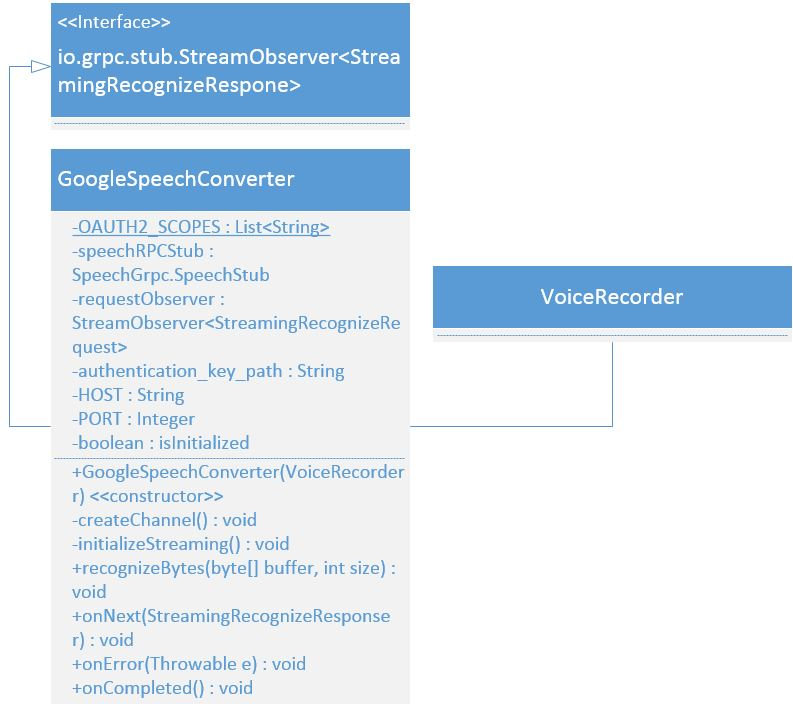
\includegraphics[width=\linewidth]{../images/GoogleSpeechConverter.JPG}
	\caption{UML Klassendiagramm der Klasse GoogleSpeechConverter}
	\label{fig:GoogleSpeechConverter}
\end{wrapfigure}
Die Funktionen bezüglich des Zugriffs auf die Google Speech API sind in der Klasse GoogleSpeechConverter im package de.dhbw.studienarbeit.hearItApp.recorder.googleSpeechRecognition gebündelt.
Der zuvor bereits thematisierte VoiceRecorder ruft im Konstruktor die private Methode initializeSpeechConverter() auf. 
Innerhalb dieser Methode wird eine neue Instanz des GoogleSpeechConverters erzeugt und dem VoiceRecorder als Attribut hinzugefügt.\\
Im Konstruktor des GoogleSpeechConverters wird ein Thread gestartet, welcher ständig die aktuelle Übertragungsgeschwindigkeit überprüft, da bei einer zu kleinen Geschwindigkeit keine Konvertierung stattfinden kann, weil Audiodaten in Echtzeit gestreamt werden müssen.\\
Danach wird durch die Methode createChannel() ein ManagedChannel nach dem bereits beschriebenen Ablauf erzeugt.
\begin{lstlisting}
 private Channel createChannel()
 	throws IOException, GeneralSecurityException {
 	
	InputStream credentials =this.recorder.getMainView()
		.getAssets().open(authentication\_key);
		
	GoogleCredentials creds = GoogleCredentials.fromStream(credentials)
		.createScoped(this.OAUTH2\_SCOPES);
		
	OkHttpChannelProvider provider = new OkHttpChannelProvider();
	OkHttpChannelBuilder builder = provider.builderForAddress(
		this.HOST, this.PORT);
	
	ManagedChannel channel = builder.intercept(
		new ClientAuthInterceptor(
		creds, Executors.newSingleThreadExecutor()))
		.build();
	
	credentials.close();
	
	return channel;
}
\end{lstlisting}
Mit diesem Channel wird ein SpeechGrpc.SpeechStub Objekt initialisiert durch die Methode SpeechGrpc.newStub(channel).\\
Wird dann eine Aufnahme gestartet, ruft der VoiceRecorder nach jedem lesen von AudioBytes die Methode recognizeBytes(byte[] buffer, int size) auf.\\
Innerhalb dieser Methode erfolgt eine Überprüfung, ob der Converter bereits initialisiert wurde. Wenn nicht, wird die Methode initializeStreaming() aufgerufen. Hier wird dem im Konstruktor initialisierten SpeechStub durch die Methode speechRPCStub.streamingRecognize(this) der ResponseStreamObserver zugewiesen.\\
Der Zugewiesene ResponseStreamObserver wird vom SpeechStub benachrichtigt, sobald eine Antwort von der SpeechAPI erhalten wird. Um als solcher zu funkieren, muss die Klasse das Interface io.grpc.stub.StreamObserver<StreamingRecognizeResponse> und die zugehörigen, selbsterklärenden Methoden onNext(StreamingRecognizeResponse response), onError( Throwable error ) und onCompleted() implementieren. Diese Methoden werden im jeweiligen Fall vom SpeechStub aufgerufen.\\
Die Methode speechRPCStub.streamingRecognize(this) gibt ein Objekt der Klasse StreamObserver<StreamingRecognizeRequest>, welches im Attribut requestObserver gespeichert wird, zurück. Über den RequestObeserver Stream können Daten an die Google API gesendet werden.\\
Sind beide Streams initialisiert, wird nach den zuvor beschriebenen API Regeln eine RecognitionConfig in eine StreamingRecognitionConfig eingebettet und daraus ein StreamingRecognizeRequest erzeugt, welches durch die Methode requestObserver.onNext(requehst) an die API gesendet wird, um die Konvertierung zu initialisieren. Der Programmcode zum generieren der Konfiguration ist im Anschluss abgebildet.
\begin{lstlisting}
RecognitionConfig audioConfig =
	RecognitionConfig.newBuilder()
		.setEncoding( RecognitionConfig.AudioEncoding.LINEAR16 )
		.setSampleRate( VoiceRecorder.SAMPLING )
		.build();

StreamingRecognitionConfig streamingConfig =
	StreamingRecognitionConfig.newBuilder()
		.setConfig( audioConfig )
		.setInterimResults( false )
		.setSingleUtterance( false )
		.build();

StreamingRecognizeRequest initialRequest =
	StreamingRecognizeRequest
		.newBuilder()
		.setStreamingConfig( streamingConfig )
		.build();
		
//send initial request with config
this.requestObserver.onNext(initialRequest);

\end{lstlisting}
Nachdem die Konvertierung nun initialisiert wurde, wird in der recognizeBytes Methode das isInitialized Flag auf true gesetzt, um eine erneute Initialisierung zu vermeiden.\\
Um die Audio Daten zu Google zu senden, wird erneut ein StreamingRecognizeRequest initialisiert. Statt einer StreamingRecognitionConfig, werden diesem aber durch die Methode setAudioContent die Übergebenen Audio Bytes zugewiesen. Durch requestObserver.onNext(request) wird der Request gesendet.

\begin{lstlisting}
public void recognizeBytes(byte[] buffer, int size){

	if (!this.isInititalized) {
		this.initializeStreaming();
		this.isInititalized = true;
	}
	try {
		StreamingRecognizeRequest request =
			StreamingRecognizeRequest.newBuilder()
				.setAudioContent(ByteString
					.copyFrom(buffer, 0, size))
				.build();
		requestObserver.onNext(request);
		
	} catch (RuntimeException e){
		Log.e(MainActivity.LOG\_TAF, "Error while recognizing speech. Stopping."
			+ e.getMessage());
		requestObserver.onError(e);
		throw e;
	}
}

\end{lstlisting}

\paragraph{Verarbeitung der Antworten}
Die Verarbeitung der Antworten, passiert im dem SpeechStub zugewiesenen ResponseStreamObserver, welcher ebenfalls in der GoogleSpeechConverter Klasse implementiert ist.\\
Bei einem Fehler wird die onError Methode mit einem Throwable als Parameter aufgerufen. Innerhalb der Methode, wird der Fehler in die Log Datei geschrieben und durch this.recorder.stopRecording() die Aufnahme beendet.\\
Bei einem positiven Ergebnis wird innerhalb der aufgerufenen onNext(StreamingRecognizeRespone respone) Methode die Liste der in der response entahltenen StreamingRecognitionResults ausgelesen. Sind Ergebnisse in der Antwort enthalten, werden vom ersten Ergebnis, welches den Index 0 hat, durch getAlternativesList() die Übersetzungsalternativen gewonnen. Die erste alternative, die die Wahrscheinlichste Übersetzung darstellt, wird durch this.recorder.getMainView().receiveResult(alternative.getTranscript()) and die MainActivity weiter geleitet, welche den ausgewählten Connector mit der Anzeige des Textes beauftragt.\\
Eine Prüfung des is\_final Flags in der Antwort ist nicht notwendig, da durch das setzen der Einstellung interrim\_results=true während der Initialisierung des Streamings sichergestellt wurde, dass alle Antworten nur finale Phrasen enthalten.


\paragraph{Überprüfung der Übertragungsgeschwindigkeit}

\paragraph{Zeitliche Analyse der Konvertierung}
\paragraph{Maximaler Streaming Zeitraum}


\section{Der TextFieldRecorder / Konvertierer}